% ============================================================
% SECTION 5: KHAI PHÁ DỮ LIỆU
% ============================================================
\section{Khai phá dữ liệu}

% --- Slide 21 ---
\begin{frame}{Phát biểu bài toán}
\begin{block}{Câu hỏi khai phá}
\textit{``Có thể dự đoán một chuyến bay sẽ trễ đến $\geq 15$ phút hay không,
chỉ dựa trên thông tin biết \textbf{trước} khi cất cánh?''}
\end{block}

\vspace{3mm}
\begin{columns}[T,onlytextwidth]
\begin{column}{0.5\textwidth}
\textbf{Bài toán phân lớp nhị phân:}
\begin{itemize}
  \item Nhãn: \texttt{is\_delayed\_15} (0/1).
  \item Mất cân bằng: 81\% / 19\%.
  \item \textbf{Không dùng} \texttt{departure\_delay}.
\end{itemize}
\end{column}
\begin{column}{0.5\textwidth}
\textbf{Quy trình end-to-end:}
\begin{enumerate}
  \item Lấy 500K mẫu (stratified theo tháng).
  \item Tiền xử lý + 10 đặc trưng.
  \item Holdout 80/20 (stratify=y).
  \item Huấn luyện 5 mô hình.
  \item Đánh giá 7 chỉ số.
\end{enumerate}
\end{column}
\end{columns}
\end{frame}

% --- Slide 22 ---
\begin{frame}{10 đặc trưng đầu vào}
\small
\begin{table}
\centering
\scriptsize
\begin{tabular}{clll}
\toprule
\textbf{Nhóm} & \textbf{Feature} & \textbf{Kiểu} & \textbf{Lý do} \\
\midrule
\multirow{4}{*}{\rotatebox{90}{\tiny Thời gian}}
  & \texttt{month}        & int   & Mùa vụ (bão hè, tuyết đông) \\
  & \texttt{day\_of\_week} & int   & Lưu lượng theo ngày \\
  & \texttt{is\_weekend}   & int   & Cờ cuối tuần \\
  & \texttt{quarter}       & int   & Quý trong năm \\
\midrule
\multirow{3}{*}{\rotatebox{90}{\tiny Chuyến}}
  & \texttt{dep\_hour}     & int   & Hiệu ứng tích lũy trong ngày \\
  & \texttt{distance}      & float & Quãng đường (dặm) \\
  & \texttt{elapsed\_time} & float & Thời gian bay (phút) \\
\midrule
\multirow{3}{*}{\rotatebox{90}{\tiny Ngữ cảnh}}
  & \texttt{airline\_enc}  & int   & Mã hãng (Label Encoding) \\
  & \texttt{origin\_enc}   & int   & Bang sân bay đi \\
  & \texttt{dest\_enc}     & int   & Bang sân bay đến \\
\bottomrule
\end{tabular}
\end{table}

\vspace{1mm}
\begin{alertblock}{Nguyên tắc quan trọng}
\small Loại \texttt{departure\_delay}, delay thành phần, \texttt{is\_cancelled}, \texttt{is\_diverted},
\texttt{tail\_number} --- tất cả chỉ biết \textit{sau} khi sự kiện xảy ra.
\end{alertblock}
\end{frame}

% --- Slide 23 ---
\begin{frame}{Cấu hình huấn luyện}
\small
\begin{table}
\centering
\scriptsize
\begin{tabular}{lp{8.5cm}}
\toprule
\textbf{Mô hình} & \textbf{Tham số chính} \\
\midrule
Logistic Regression & \texttt{saga}, C=1.0, \texttt{class\_weight='balanced'}, max\_iter=200 \\
Random Forest & 100 cây, max\_depth=10, min\_samples\_leaf=50, \texttt{class\_weight='balanced'} \\
Neural Network & [10$\to$64$\to$32$\to$1], ReLU, Adam, $\alpha$=0.001 (L2), batch=512, early stop \\
XGBoost & 300 cây, max\_depth=6, lr=0.05, subsample=0.8, \texttt{scale\_pos\_weight}$\approx$3.76 \\
LightGBM & 300 cây, max\_depth=6, lr=0.05, subsample=0.8, \texttt{is\_unbalance=True} \\
\bottomrule
\end{tabular}
\end{table}

\vspace{2mm}
\begin{block}{Xử lý mất cân bằng}
Dùng \textbf{trọng số lớp} (\texttt{class\_weight}, \texttt{scale\_pos\_weight}, \texttt{is\_unbalance})
thay vì over/undersampling $\to$ giữ nguyên phân phối gốc, tránh overfitting.
\end{block}
\end{frame}

% --- Slide 24 ---
\begin{frame}{Kết quả so sánh mô hình}
\small
\begin{table}
\centering
\begin{tabular}{lcccccc}
\toprule
\textbf{Mô hình} & \textbf{AUC} & \textbf{Acc.} & \textbf{F1} & \textbf{Avg.P} & \textbf{Log Loss} & \textbf{TG (s)} \\
\midrule
Logistic Regression & 0.6978 & 0.6570 & 0.6914 & 0.4120 & 0.6233 & \textbf{2.7} \\
Random Forest       & 0.7130 & 0.6375 & 0.6756 & 0.4107 & 0.6216 & 13.0 \\
Neural Network      & 0.7342 & \textbf{0.8318} & \textbf{0.7877} & 0.4809 & \textbf{0.4197} & 33.5 \\
XGBoost             & \textbf{0.7545} & 0.7054 & 0.7324 & \textbf{0.5078} & 0.5721 & 7.1 \\
LightGBM            & 0.7509 & 0.7031 & 0.7305 & 0.5014 & 0.5770 & 4.1 \\
\bottomrule
\end{tabular}
\end{table}

\vspace{2mm}
\begin{itemize}
  \item \textbf{XGBoost} dẫn đầu AUC-ROC (0,7545) và Avg. Precision (0,5078).
  \item \textbf{LightGBM} sát sau nhưng nhanh hơn đáng kể (4,1s vs. 7,1s).
  \item \textbf{Neural Network}: Accuracy/F1 cao nhất nhưng AUC thứ 3 --- thiên về lớp đa số.
\end{itemize}
\end{frame}

% --- Slide 25 ---
\begin{frame}{Confusion Matrix}
\centering
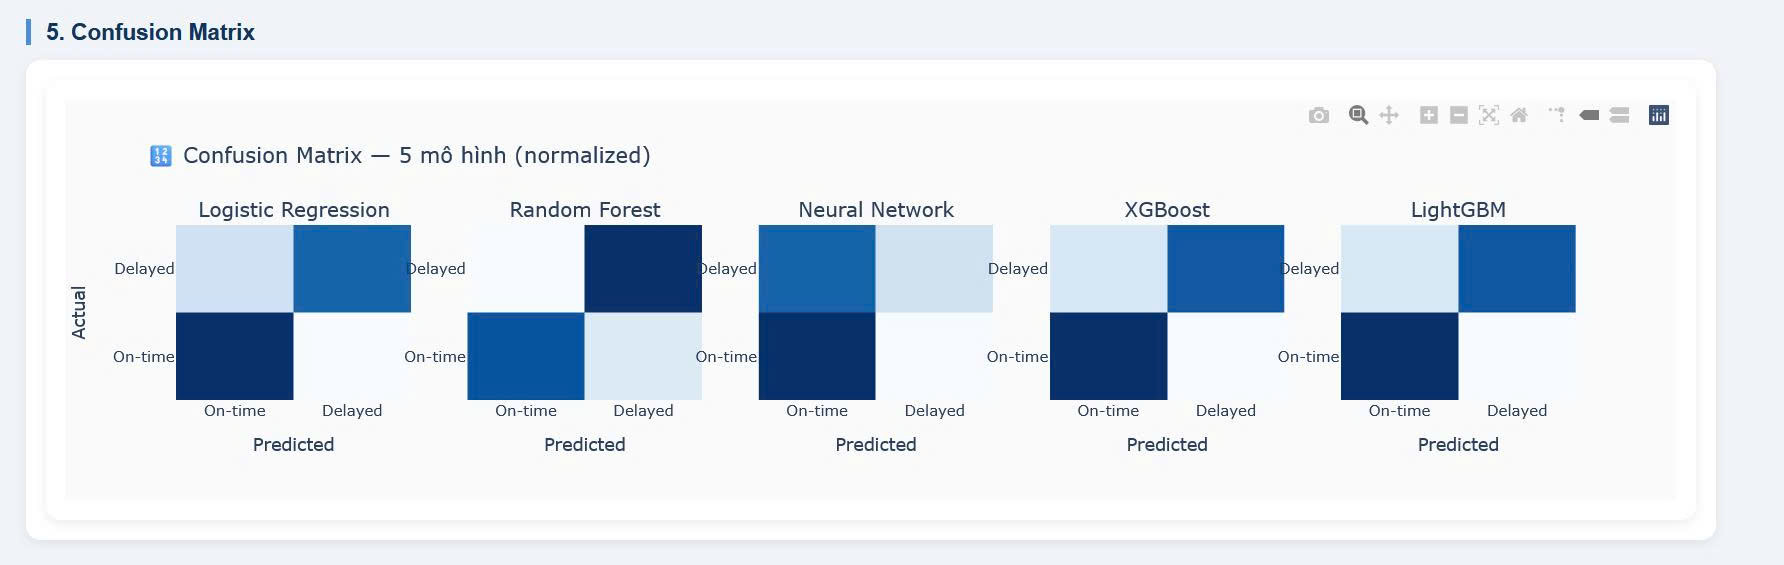
\includegraphics[width=\linewidth,keepaspectratio]{confusion_matrix.jpg}
\end{frame}

\begin{frame}{Confusion Matrix}
\textbf{LR \& RF:}\\
4 ô đồng đều --- chưa phân biệt rõ 2 lớp. AUC thấp nhất nhóm.

\vspace{2mm}
\textbf{Neural Network:}\\
True Negative rất đậm, nhưng False Negative cao $\to$ \textbf{bỏ sót delay}.
Accuracy 0,83 ``che giấu'' thiên lệch.

\vspace{2mm}
\textbf{XGBoost \& LightGBM:}\\
Đường chéo \textbf{cân đối nhất} --- phân biệt tốt \textit{cả hai lớp}.

\vspace{2mm}
\begin{alertblock}{}
\small Accuracy đơn thuần \textbf{gây hiểu nhầm} khi dữ liệu mất cân bằng.
\end{alertblock}
\end{frame}

% --- Slide 26 ---
\begin{frame}{Feature Importance}
\centering
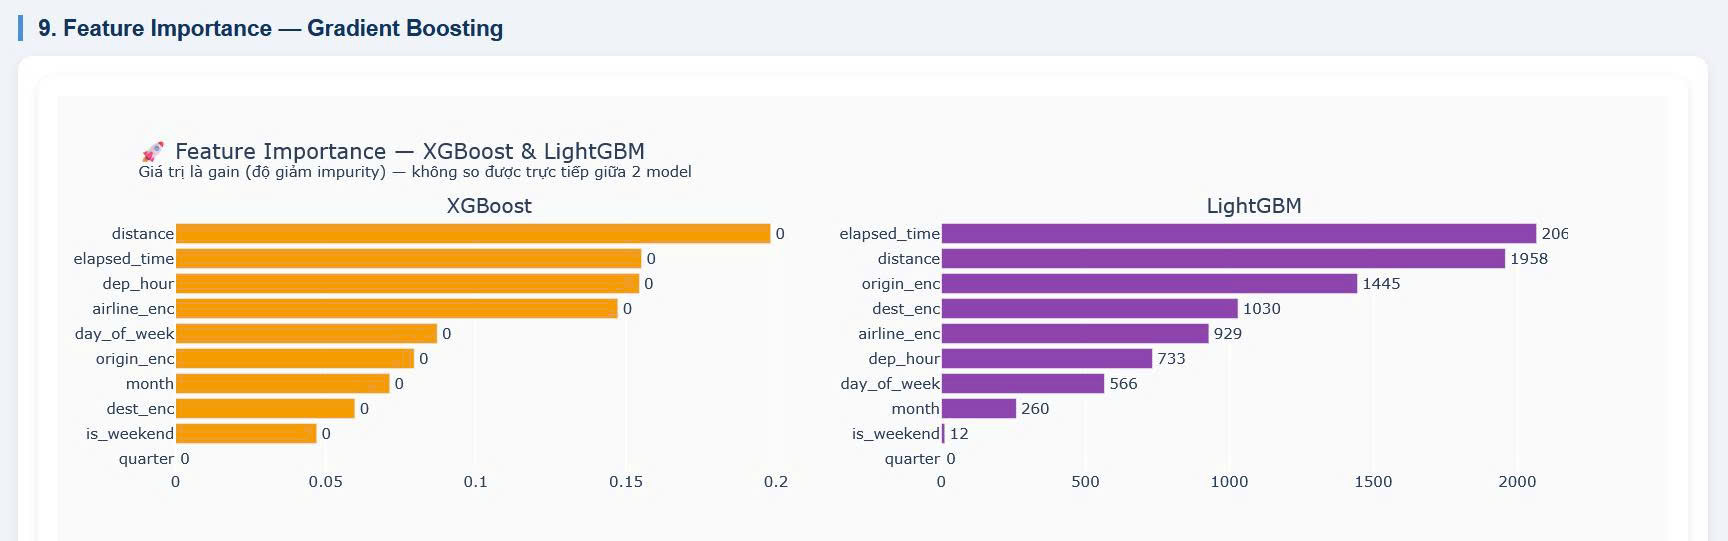
\includegraphics[width=\linewidth,keepaspectratio]{feature_importance.jpg}
\end{frame}

\begin{frame}{Feature Importance}
\textbf{Top features (cả 2 model):}
\begin{enumerate}
  \item \texttt{distance} \& \texttt{elapsed\_time}\\
        Chuyến dài = nhiều rủi ro hơn.
  \item \texttt{dep\_hour}\\
        Hiệu ứng tích lũy chiều/tối.
  \item \texttt{airline\_enc}\\
        OTP chênh 15--20\% giữa hãng.
  \item \texttt{origin/dest\_enc}\\
        Yếu tố địa lý quan trọng.
\end{enumerate}

\vspace{2mm}
\texttt{is\_weekend}, \texttt{quarter} thấp nhất
$\to$ đã ``bao hàm'' bởi \texttt{day\_of\_week}, \texttt{month}.

\vspace{2mm}
\textbf{Nhất quán với OLAP}: dashboard phát hiện xu hướng vĩ mô,
model lượng hóa đóng góp.
\end{frame}

% --- Slide 27 ---
\begin{frame}{Tại sao Gradient Boosting tốt nhất?}
\begin{enumerate}
  \item \textbf{Nắm bắt quan hệ phi tuyến}\\
        Delay vs. đặc trưng không tuyến tính --- LR không biểu diễn được.

  \item \textbf{Tự phát hiện interaction features}\\
        VD: hãng F9 + tháng 12 + sân bay ORD $\to$ delay cao.

  \item \textbf{Boosting tuần tự vs. Bagging song song}\\
        Mỗi cây sửa lỗi cây trước $\to$ hội tụ tốt hơn RF.

  \item \textbf{Xử lý mất cân bằng lớp tích hợp}\\
        \texttt{scale\_pos\_weight}, \texttt{is\_unbalance} điều chỉnh gradient theo tỷ lệ lớp.

  \item \textbf{LightGBM: tốc độ vượt trội}\\
        Leaf-wise + histogram: 4,1s vs. 7,1s, chỉ thua 0,004 AUC.
\end{enumerate}
\end{frame}

% --- Slide 28 ---
\begin{frame}{Những trường hợp mô hình còn sai}
Dù Gradient Boosting tốt nhất, AUC $\approx$ 0,75 vẫn còn khoảng cách:

\vspace{3mm}
\begin{columns}[T,onlytextwidth]
\begin{column}{0.48\textwidth}
\begin{block}{Nguyên nhân sai}
\begin{itemize}
  \item \textbf{Thời tiết cực đoan} đột xuất\\
        (bão tuyết, mưa đá bất ngờ).
  \item \textbf{Delay vận hành nội bộ}\\
        (thiếu phi hành đoàn, bảo trì đột xuất).
\end{itemize}
\end{block}
\end{column}
\begin{column}{0.48\textwidth}
\begin{block}{Nguyên nhân sai (tt.)}
\begin{itemize}
  \item \textbf{Sân bay/hãng ít dữ liệu}\\
        Encoding không đại diện.
  \item \textbf{Ngày lễ đặc biệt}\\
        Thanksgiving, Giáng sinh: hành vi delay khác biệt.
\end{itemize}
\end{block}
\end{column}
\end{columns}

\vspace{3mm}
$\Rightarrow$ Gợi ý: tích hợp dữ liệu thời tiết, thêm feature ngày lễ.
\end{frame}
